% ===========================================================
%  Preparatório OBI — Algoritmos Gulosos (Greedy)
%  Grupo: GEMA
%  Compilar: pdflatex aula_greedy.tex  (rodar 2x)
% ===========================================================
\documentclass[aspectratio=169,10pt]{beamer}

\usetheme{Madrid}
\usecolortheme{default}

% ── Pacotes ─────────────────────────────────────────────────
\usepackage[utf8]{inputenc}
\usepackage[T1]{fontenc}
\usepackage[english]{babel}
\usepackage{graphicx}
\usepackage{listings}
\usepackage{xcolor}
\usepackage{tikz}
\usepackage{amsmath}
\usepackage{amssymb}
\usepackage{tcolorbox}
\usepackage{array}
\usepackage{booktabs}
\usepackage{adjustbox}
\usepackage{colortbl}
\tcbuselibrary{skins,breakable,listings}
\usetikzlibrary{arrows.meta,shapes,positioning,fit,calc,
                decorations.pathreplacing,backgrounds,patterns}

% ── Margens ─────────────────────────────────────────────────
\setbeamersize{text margin left=4mm,text margin right=4mm}
\setlength{\leftmargini}{1.0em}
\setlength{\leftmarginii}{0.9em}

% ── Paleta de Cores ─────────────────────────────────────────
\definecolor{gemaBlue}    {RGB}{13,   43,  90}
\definecolor{gemaCyan}    {RGB}{0,   170, 210}
\definecolor{gemaRed}     {RGB}{190,  30,  30}
\definecolor{gemaOrange}  {RGB}{220, 110,   0}
\definecolor{gemaGreen}   {RGB}{30,  150,  70}
\definecolor{gemaGold}    {RGB}{200, 160,   0}
\definecolor{gemaPurple}  {RGB}{120,   0, 160}
\definecolor{codeBack}    {RGB}{22,   27,  34}
\definecolor{codeGreen}   {RGB}{80,  200, 120}
\definecolor{codeBlue}    {RGB}{121, 192, 255}
\definecolor{codeYellow}  {RGB}{255, 210,  70}
\definecolor{codeOrange}  {RGB}{255, 160,  60}
\definecolor{alertYellow} {RGB}{255, 243, 176}
\definecolor{alertBorder} {RGB}{160, 110,   0}
\definecolor{greedyGold}  {RGB}{215, 175,   0}
\definecolor{stepBlue}    {RGB}{40,  100, 200}
\definecolor{stepGreen}   {RGB}{20,  140,  60}
\definecolor{stepRed}     {RGB}{200,  40,  40}

% ── Cores Beamer ────────────────────────────────────────────
\setbeamercolor{palette primary}    {bg=gemaBlue,  fg=white}
\setbeamercolor{palette secondary}  {bg=gemaBlue!85,fg=white}
\setbeamercolor{palette tertiary}   {bg=gemaBlue!65,fg=white}
\setbeamercolor{palette quaternary} {bg=gemaBlue,  fg=white}
\setbeamercolor{structure}          {fg=gemaBlue}
\setbeamercolor{frametitle}         {fg=white, bg=gemaBlue}
\setbeamercolor{block title}        {fg=white, bg=gemaBlue}
\setbeamercolor{block body}         {fg=black, bg=gemaBlue!7}
\setbeamercolor{block title alerted}{fg=white, bg=gemaRed}
\setbeamercolor{block body alerted} {fg=black, bg=gemaRed!8}
\setbeamercolor{block title example}{fg=white, bg=gemaGreen!75!black}
\setbeamercolor{block body example} {fg=black, bg=gemaGreen!10}
\setbeamercolor{itemize item}       {fg=gemaCyan!70!black}
\setbeamercolor{itemize subitem}    {fg=gemaBlue!60}

\setbeamerfont{frametitle}{size=\large, series=\bfseries}
\setbeamertemplate{navigation symbols}{}

% ── Rodapé ──────────────────────────────────────────────────
\setbeamertemplate{footline}{%
  \leavevmode\hbox{%
    \begin{beamercolorbox}[wd=.33\paperwidth,ht=2.8ex,dp=1.2ex,center]{palette secondary}
      \tiny GEMA
    \end{beamercolorbox}%
    \begin{beamercolorbox}[wd=.34\paperwidth,ht=2.8ex,dp=1.2ex,center]{palette primary}
      \tiny Algoritmos Gulosos
    \end{beamercolorbox}%
    \begin{beamercolorbox}[wd=.33\paperwidth,ht=2.8ex,dp=1.2ex,right]{palette secondary}
      \tiny \insertframenumber/\inserttotalframenumber\hspace{2mm}
    \end{beamercolorbox}%
  }%
}

% ── Estilos de Código C++ ───────────────────────────────────
\lstdefinestyle{cppstyle}{
  language=C++,
  backgroundcolor=\color{codeBack},
  basicstyle=\ttfamily\scriptsize\color{white},
  keywordstyle=\color{codeBlue}\bfseries,
  stringstyle=\color{codeOrange},
  commentstyle=\color{codeGreen}\itshape,
  numberstyle=\tiny\color{gray!60},
  identifierstyle=\color{white},
  morekeywords={vector,pair,sort,priority_queue,greater,auto,bool,
                long,string,int64\_t,size\_t},
  emph={push\_back,push,pop,top,front,empty,size,make\_pair,
        first,second,begin,end,cout,cin,endl,min,max},
  emphstyle=\color{codeYellow}\bfseries,
  numbers=left, numbersep=5pt,
  frame=none, tabsize=4,
  showstringspaces=false,
  breaklines=true, columns=flexible, keepspaces=true,
  xleftmargin=10pt, aboveskip=0pt, belowskip=0pt,
}

\lstdefinestyle{cppsmall}{
  style=cppstyle,
  basicstyle=\ttfamily\tiny\color{white},
  numberstyle=\tiny\color{gray!50},
  numbersep=3pt, xleftmargin=7pt, lineskip=-0.5pt,
}

% ── Caixas tcolorbox ────────────────────────────────────────
\tcbset{
  before skip=1pt, after skip=1pt, boxsep=0pt,
  caixaBase/.style={enhanced,arc=4pt,boxrule=0.8pt,
    left=3pt,right=3pt,top=2pt,bottom=2pt,
    fonttitle=\bfseries\footnotesize},
  caixaAzul/.style={caixaBase,
    colback=gemaBlue!6,colframe=gemaBlue},
  caixaVerde/.style={caixaBase,
    colback=gemaGreen!8,colframe=gemaGreen!60!black,
    fonttitle=\bfseries\footnotesize\color{gemaGreen!35!black}},
  caixaVermelho/.style={caixaBase,
    colback=gemaRed!8,colframe=gemaRed,
    fonttitle=\bfseries\footnotesize\color{gemaRed!80!black}},
  caixaLaranja/.style={caixaBase,
    colback=gemaOrange!8,colframe=gemaOrange,
    fonttitle=\bfseries\footnotesize\color{gemaOrange!80!black}},
  caixaDourada/.style={caixaBase,
    colback=greedyGold!10,colframe=greedyGold,
    fonttitle=\bfseries\footnotesize\color{greedyGold!70!black}},
  caixaRoxa/.style={caixaBase,
    colback=gemaPurple!8,colframe=gemaPurple!70,
    fonttitle=\bfseries\footnotesize\color{gemaPurple!70!black}},
  caixaAmarelo/.style={caixaBase,
    colback=alertYellow,colframe=alertBorder,
    fonttitle=\bfseries\footnotesize\color{alertBorder}},
  caixaCodigo/.style={enhanced,arc=4pt,boxrule=0.8pt,
    colback=codeBack,colframe=gemaCyan!45,
    left=1pt,right=1pt,top=1pt,bottom=1pt},
}

% ── Metadados ───────────────────────────────────────────────
\title[Greedy --- Algoritmos Gulosos]{Algoritmos Gulosos (Greedy)}
\subtitle{Preparatorio OBI --- Aula 04}
\author[GEMA]{Grupo de Extensao em Maratonas de Programação}
\institute{GEMA}
\date{2025}

% ============================================================
\begin{document}
% ============================================================

% ── SLIDE DE TITULO ─────────────────────────────────────────
{
\setbeamertemplate{footline}{}
\begin{frame}[noframenumbering]
  \begin{columns}[c]
    \column{0.62\textwidth}
      \vspace{0.2cm}
      {\fontsize{20}{24}\selectfont\bfseries\color{gemaBlue}
        Algoritmos Gulosos\par}
      \vspace{0.1cm}
      {\fontsize{14}{17}\selectfont\color{greedyGold}\bfseries
        Greedy Algorithms\par}
      \vspace{0.15cm}
      {\large\color{gemaCyan} Preparatório OBI --- Aula 04\par}
      \vspace{0.35cm}

    \column{0.36\textwidth}
      \centering
      
\includegraphics[width=0.50\linewidth]{logo.png}\\[0.3cm]
      
\includegraphics[width=0.50\linewidth]{logo_obi.png}
  \end{columns}
\end{frame}
}

% ── AGENDA ──────────────────────────────────────────────────
\begin{frame}{Agenda}
  \begin{columns}[t]
    \column{0.48\textwidth}
      \begin{block}{Fundamentos}
        \begin{enumerate}\footnotesize
          \item O que e um algoritmo guloso?
          \item Intuição da estratégia
          \item Propriedades que garantem corretude
          \item Quando o guloso falha?
        \end{enumerate}
      \end{block}
      \vspace{0.15cm}
      \begin{block}{Exemplos clássicos}
        \begin{enumerate}\setcounter{enumi}{4}\footnotesize
          \item Troco com moedas
          \item Interval Scheduling
          \item Plataformas / Salas
          \item Fractional Knapsack
        \end{enumerate}
      \end{block}
    \column{0.48\textwidth}
      \begin{block}{Técnicas e práticas}
        \begin{enumerate}\setcounter{enumi}{8}\footnotesize
          \item Estrategias comuns em gulosos
          \item Como identificar na OBI
          \item Armadilhas e erros comuns
          \item Problemas para praticar
        \end{enumerate}
      \end{block}
      \vspace{0.15cm}
      \begin{tcolorbox}[caixaDourada,title={Meta da aula}]
        \footnotesize
        Reconhecer quando o guloso funciona
        e \textbf{provar} intuitivamente por que
        a escolha local leva ao ótimo global.
      \end{tcolorbox}
  \end{columns}
\end{frame}

% ============================================================
%  PARTE 1 — FUNDAMENTOS
% ============================================================
{
\setbeamertemplate{footline}{}
\begin{frame}[noframenumbering]
  \centering\vspace{1.0cm}
  {\fontsize{36}{44}\selectfont\bfseries\color{gemaBlue} 1}\par
  \vspace{0.25cm}
  {\Large\color{greedyGold}\bfseries Fundamentos}\par
  \vspace{0.15cm}
  {\color{gray}\small O que e? Como pensar? Quando funciona?}
\end{frame}
}

% ── O QUE E UM ALGORITMO GULOSO ─────────────────────────────
\begin{frame}{O que e um Algoritmo Guloso?}
  \begin{columns}[c]
    \column{0.50\textwidth}
      \begin{tcolorbox}[caixaDourada,title={Definição}]
        \small
        Um algoritmo guloso constroi a solução
        \textbf{passo a passo}, sempre escolhendo
        a opção que parece \textbf{melhor naquele momento},
        sem revisitar decisoes anteriores.
      \end{tcolorbox}
      \vspace{0.12cm}
      \begin{tcolorbox}[caixaAzul,title={Características}]
        \begin{itemize}\footnotesize
          \item Toma \textbf{uma decisao por vez}
          \item Nunca \textbf{volta atras}
          \item Rapido: geralmente \textbf{O(n log n)}
          \item Pode ou nao ser \textbf{ótimo global}
        \end{itemize}
      \end{tcolorbox}
      \vspace{0.12cm}
      \begin{tcolorbox}[caixaVermelho,title={Diferença crucial}]
        \footnotesize
        Guloso $\neq$ Força bruta e $\neq$ DP.\\
        O guloso \textbf{nunca testa todas as opções}.
      \end{tcolorbox}
    \column{0.48\textwidth}
      \centering
      % Diagrama: caminhante escolhendo sempre o maior pico visivel
      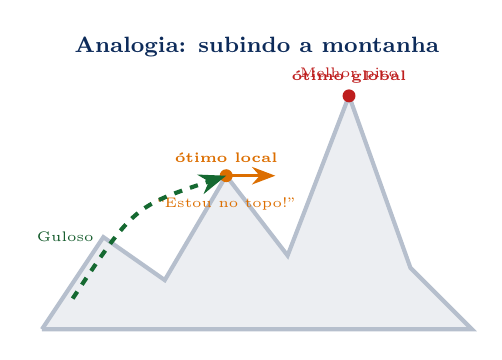
\begin{tikzpicture}[scale=0.78]
        % Titulo
        \node[font=\bfseries\footnotesize,gemaBlue] at (3.5,4.6)
          {Analogia: subindo a montanha};
        % Terreno
        \draw[gemaBlue!30,line width=1.5pt,fill=gemaBlue!8]
          (0,0)--(1,1.5)--(2,0.8)--(3,2.5)--(4,1.2)--(5,3.8)--(6,1.0)--(7,0)--(7,0)--(0,0);
        % Picos
        \node[font=\tiny,gemaRed] at (5,4.1){\textbf{ótimo global}};
        \node[font=\tiny,gemaOrange] at (3,2.8){\textbf{ótimo local}};
        % Personagem no ótimo local
        \fill[gemaOrange] (3,2.5) circle (3pt);
        \draw[-{Stealth},gemaOrange,line width=1.2pt](3,2.5)--(3.8,2.5);
        \node[font=\tiny,gemaOrange,below] at (3,2.3){``Estou no topo!''};
        % Personagem no ótimo global
        \fill[gemaRed] (5,3.8) circle (3pt);
        \node[font=\tiny,gemaRed,above] at (5,3.9){Melhor pico};
        % Seta guloso
        \draw[-{Stealth},gemaGreen!70!black,line width=1.5pt,dashed]
          (0.5,0.5) .. controls (1.5,2.0) .. (3,2.5);
        \node[font=\tiny,gemaGreen!60!black,left] at (1.0,1.5){Guloso};
      \end{tikzpicture}
      \vspace{0.1cm}
      \begin{tcolorbox}[caixaAmarelo,title={}]
        \footnotesize
        O guloso sobe sempre o próximo degrau
        mais alto. Pode chegar no ótimo global
        \textbf{ou parar num ótimo local}.
      \end{tcolorbox}
  \end{columns}
\end{frame}

% ── INTUIção: COMPARAção ────────────────────────────────────
\begin{frame}{Guloso vs Forca Bruta vs Programação dinâmica}
  \centering
  \begin{adjustbox}{max totalsize={0.97\textwidth}{0.78\textheight},center}
  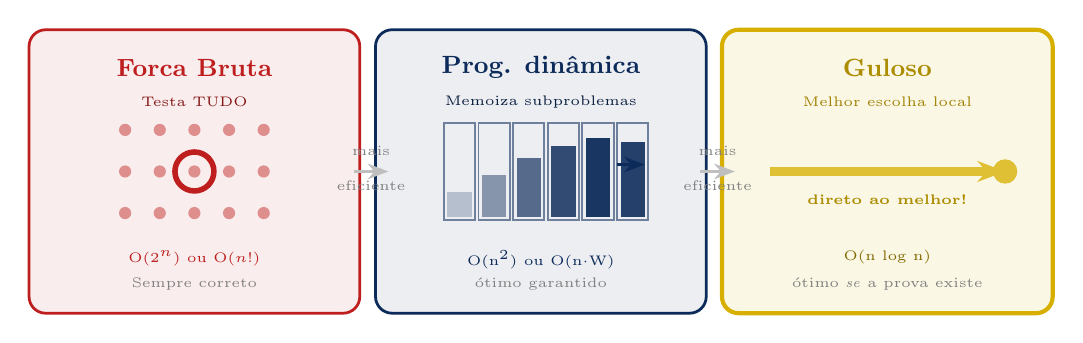
\begin{tikzpicture}[scale=0.88]

    % ── FORCA BRUTA ───────────────────────────────────────
    \node[draw=gemaRed,fill=gemaRed!8,rounded corners=6pt,
          minimum width=4.2cm,minimum height=3.6cm,line width=1pt]
          at (2.2,2.2){};
    \node[font=\bfseries\small,gemaRed] at (2.2,3.7){Forca Bruta};
    \node[font=\tiny,align=center,gemaRed!70!black] at (2.2,3.2){Testa TUDO};
    % Grid de possibilidades
    \foreach \x/\y in {1.2/2.8,1.7/2.8,2.2/2.8,2.7/2.8,3.2/2.8,
                        1.2/2.2,1.7/2.2,2.2/2.2,2.7/2.2,3.2/2.2,
                        1.2/1.6,1.7/1.6,2.2/1.6,2.7/1.6,3.2/1.6}{
      \fill[gemaRed!50] (\x,\y) circle (2.5pt);
    }
    \draw[gemaRed,line width=2pt] (2.2,2.2) circle (8pt);
    \node[font=\tiny,gemaRed,below] at (2.2,1.2){O($2^n$) ou O($n!$)};
    \node[font=\tiny,gray,below] at (2.2,0.8){Sempre correto};

    % ── DP ─────────────────────────────────────────────────
    \node[draw=gemaBlue,fill=gemaBlue!8,rounded corners=6pt,
          minimum width=4.2cm,minimum height=3.6cm,line width=1pt]
          at (7.2,2.2){};
    \node[font=\bfseries\small,gemaBlue] at (7.2,3.7){Prog. dinâmica};
    \node[font=\tiny,align=center,gemaBlue!70!black] at (7.2,3.2){Memoiza subproblemas};
    % Tabela DP
    \foreach \x/\y in {5.8/2.8,6.3/2.8,6.8/2.8,7.3/2.8,7.8/2.8,8.3/2.8}{
      \draw[gemaBlue!60,line width=0.7pt] (\x,1.5) rectangle (\x+0.45,2.9);
    }
    \foreach \x/\c in {5.8/30,6.3/50,6.8/70,7.3/85,7.8/95,8.3/90}{
      \fill[gemaBlue!\c] (\x+0.05,1.55) rectangle (\x+0.4,1.55+\c*0.012);
    }
    \draw[-{Stealth},gemaBlue,line width=1pt](8.3,2.3)--(8.7,2.3);
    \node[font=\tiny,gemaBlue,below] at (7.2,1.2){O(n$^2$) ou O(n$\cdot$W)};
    \node[font=\tiny,gray,below] at (7.2,0.8){ótimo garantido};

    % ── GULOSO ─────────────────────────────────────────────
    \node[draw=greedyGold,fill=greedyGold!10,rounded corners=6pt,
          minimum width=4.2cm,minimum height=3.6cm,line width=1.5pt]
          at (12.2,2.2){};
    \node[font=\bfseries\small,greedyGold!80!black] at (12.2,3.7){Guloso};
    \node[font=\tiny,align=center,gemaGold!80!black] at (12.2,3.2){Melhor escolha local};
    % Seta reta para o melhor
    \draw[-{Stealth[length=10pt]},greedyGold!80,line width=3pt]
      (10.5,2.2)--(13.9,2.2);
    \fill[greedyGold!80] (13.9,2.2) circle (5pt);
    \node[font=\bfseries\tiny,greedyGold!80!black] at (12.2,1.8){direto ao melhor!};
    \node[font=\tiny,greedyGold!60!black,below] at (12.2,1.2){O(n log n)};
    \node[font=\tiny,gray,below] at (12.2,0.8){ótimo \textit{se} a prova existe};

    % Setas de comparação
    \draw[-{Stealth},gray!50,line width=1pt](4.5,2.2)--(5.0,2.2);
    \node[font=\tiny,gray] at (4.75,2.5){mais};
    \node[font=\tiny,gray] at (4.75,2.0){eficiente};
    \draw[-{Stealth},gray!50,line width=1pt](9.5,2.2)--(10.0,2.2);
    \node[font=\tiny,gray] at (9.75,2.5){mais};
    \node[font=\tiny,gray] at (9.75,2.0){eficiente};

  \end{tikzpicture}
  \end{adjustbox}
\end{frame}

% ── PROPRIEDADES DO GULOSO ──────────────────────────────────
\begin{frame}{Quando o Guloso Funciona? --- As Duas Propriedades}
  \begin{columns}[t]
    \column{0.48\textwidth}
      \begin{tcolorbox}[caixaDourada,title={1. Greedy Choice Property}]
        \small
        Existe sempre uma \textbf{escolha gulosa}
        (localmente otima) que faz parte de uma
        solução otima global.\\[4pt]
        Em outras palavras:\\
        \textit{``A melhor escolha agora nao estraga o futuro.''}
      \end{tcolorbox}
      \vspace{0.12cm}
      \begin{tcolorbox}[caixaAzul,title={2. Optimal Substructure}]
        \small
        Apos fazer a escolha gulosa, o subproblema
        restante tambem tem estrutura otima.\\[4pt]
        Igual a DP, mas \textbf{so há um subproblema}
        a resolver (o guloso elimina os outros).
      \end{tcolorbox}
    \column{0.50\textwidth}
      \begin{tcolorbox}[caixaVerde,title={Como provar intuitivamente?}]
        \footnotesize
        Tecnica de \textbf{exchange argument}:\\[3pt]
        \begin{enumerate}\footnotesize
          \item Assuma que existe uma solução otima
                que \textbf{nao} comeca com a escolha gulosa
          \item Mostre que voce pode \textbf{trocar}
                essa escolha pela gulosa sem piorar
          \item Logo, a escolha gulosa tambem e otima
        \end{enumerate}
      \end{tcolorbox}
      \vspace{0.1cm}
      \begin{tcolorbox}[caixaVermelho,title={Atenção}]
        \footnotesize
        Nem todo problema tem essas propriedades!\\[3pt]
        Se nao tiver: use \textbf{DP} ou \textbf{busca completa}.\\[3pt]
        Contraexemplo com moedas \{1,3,4\} e troco=6:\\
        Guloso: 4+1+1=3 moedas \textcolor{gemaRed}{(\textbf{errado})}\\
        ótimo: 3+3=2 moedas \textcolor{gemaGreen}{(\textbf{correto})}
      \end{tcolorbox}
  \end{columns}
\end{frame}

% ============================================================
%  PARTE 2 — EXEMPLOS CLASSICOS
% ============================================================
{
\setbeamertemplate{footline}{}
\begin{frame}[noframenumbering]
  \centering\vspace{1.0cm}
  {\fontsize{36}{44}\selectfont\bfseries\color{gemaBlue} 2}\par
  \vspace{0.25cm}
  {\Large\color{greedyGold}\bfseries Exemplos Classicos}\par
  \vspace{0.15cm}
  {\color{gray}\small Troco $\cdot$ Intervalos $\cdot$ Salas $\cdot$ Mochila}
\end{frame}
}

% ── EXEMPLO 1: TROCO ────────────────────────────────────────
\begin{frame}{Exemplo 1 --- Troco com Moedas (onde o guloso funciona)}
  \begin{columns}[c]
    \column{0.50\textwidth}
      \begin{tcolorbox}[caixaAzul,title={Problema}]
        \small
        Moedas disponiveis: \textbf{25, 10, 5, 1} centavos.\\
        Dar troco de \textbf{R\$ 0,41} com o
        \textbf{menor numero} de moedas.
      \end{tcolorbox}
      \vspace{0.1cm}
      \textbf{\small Estrategia gulosa:}\\
      \footnotesize Use sempre a \textbf{maior moeda possivel}.
      \vspace{0.12cm}

      % Passo a passo
      \begin{tcolorbox}[caixaVerde,title={Passo a Passo}]
        \footnotesize
        \begin{tabular}{clr}
          \toprule
          Passo & Moeda usada & Restante\\
          \midrule
          1 & 25c & 16c\\
          2 & 10c & 6c\\
          3 & 5c  & 1c\\
          4 & 1c  & 0c\\
          \bottomrule
        \end{tabular}\\[4pt]
        \textbf{Total: 4 moedas} \textcolor{gemaGreen}{$\checkmark$}
      \end{tcolorbox}
    \column{0.48\textwidth}
      \centering
      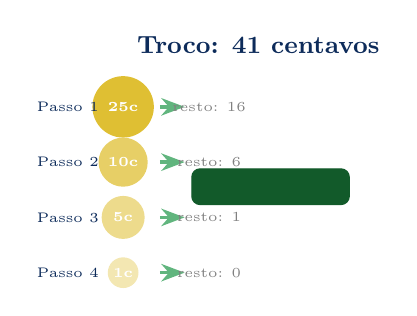
\begin{tikzpicture}[scale=0.78]
        % Moedas visuais
        \node[font=\bfseries\small,gemaBlue] at (3.0,4.5){Troco: 41 centavos};

        % Moeda 25
        \fill[greedyGold!80] (0.8,3.5) circle (0.5);
        \node[font=\bfseries\tiny,white] at (0.8,3.5){25c};
        \draw[-{Stealth},gemaGreen!70,line width=1.2pt](1.4,3.5)--(1.8,3.5);
        \node[font=\tiny,gray] at (2.2,3.5){resto: 16};

        % Moeda 10
        \fill[greedyGold!60] (0.8,2.6) circle (0.4);
        \node[font=\bfseries\tiny,white] at (0.8,2.6){10c};
        \draw[-{Stealth},gemaGreen!70,line width=1.2pt](1.4,2.6)--(1.8,2.6);
        \node[font=\tiny,gray] at (2.2,2.6){resto: 6};

        % Moeda 5
        \fill[greedyGold!45] (0.8,1.7) circle (0.35);
        \node[font=\bfseries\tiny,white] at (0.8,1.7){5c};
        \draw[-{Stealth},gemaGreen!70,line width=1.2pt](1.4,1.7)--(1.8,1.7);
        \node[font=\tiny,gray] at (2.2,1.7){resto: 1};

        % Moeda 1
        \fill[greedyGold!30] (0.8,0.8) circle (0.25);
        \node[font=\bfseries\tiny,white] at (0.8,0.8){1c};
        \draw[-{Stealth},gemaGreen!70,line width=1.2pt](1.4,0.8)--(1.8,0.8);
        \node[font=\tiny,gray] at (2.2,0.8){resto: 0};

        % Resultado
        \node[draw=gemaGreen,fill=gemaGreen!10,rounded corners=3pt,
              font=\bfseries\small,gemaGreen!60!black,
              minimum width=2.0cm] at (3.2,2.2){4 moedas};

        % Label passos
        \foreach \y/\n in {3.5/1, 2.6/2, 1.7/3, 0.8/4}{
          \node[font=\tiny,gemaBlue] at (-0.1,\y){Passo \n};
        }
      \end{tikzpicture}
      \begin{tcolorbox}[caixaAmarelo,title={Por que funciona aqui?}]
        \footnotesize
        Moedas \{1,5,10,25\} sao \textbf{multiplos} e
        cada grande cobre exatamente $k$ pequenas.
        O exchange argument garante otimalidade.
      \end{tcolorbox}
  \end{columns}
\end{frame}

% ── EXEMPLO 1: CÓDIGO ───────────────────────────────────────
\begin{frame}[fragile,shrink=3]{Exemplo 1 --- Codigo C++: Troco com Moedas}
  \begin{columns}[t]
    \column{0.58\textwidth}
      \begin{tcolorbox}[caixaCodigo]
        \begin{lstlisting}[style=cppstyle]
#include <bits/stdc++.h>
using namespace std;

int main(){
    // Moedas em ordem DECRESCENTE (chave do guloso)
    vector<int> moedas = {25, 10, 5, 1};
    int troco;
    cin >> troco;

    int total = 0;
    vector<pair<int,int>> usado; // {moeda, qtd}

    for(int m : moedas){
        if(troco >= m){
            int qtd = troco / m;   // quantas cabem
            troco   = troco % m;   // restante
            usado.push_back({m, qtd});
            total += qtd;
        }
    }

    cout << "Moedas usadas: " << total << "\n";
    for(auto [m, q] : usado)
        cout << q << " moeda(s) de " << m << "c\n";

    return 0;
}
        \end{lstlisting}
      \end{tcolorbox}
    \column{0.40\textwidth}
      \begin{tcolorbox}[caixaDourada,title={Chave do Guloso}]
        \footnotesize
        Ordenar moedas em ordem
        \textbf{decrescente} e sempre
        usar a maior que cabe.\\[4pt]
        A ordenação e O(k) para
        k moedas fixas.
      \end{tcolorbox}
      \vspace{0.1cm}
      \begin{tcolorbox}[caixaAzul,title={Complexidade}]
        \footnotesize
        \textbf{Tempo:} O(k)\\
        k = numero de tipos de moedas\\[3pt]
        \textbf{Espaco:} O(k)
      \end{tcolorbox}
      \vspace{0.1cm}
      \begin{tcolorbox}[caixaVermelho,title={Contraexemplo!}]
        \footnotesize
        Moedas \{1, 3, 4\}, troco=6:\\[2pt]
        Guloso: 4+1+1 = \textbf{3 moedas}\\
        ótimo:  3+3 = \textbf{2 moedas}\\[2pt]
        Nesse sistema: \textbf{use DP!}
      \end{tcolorbox}
  \end{columns}
\end{frame}

% ── CONTRAEXEMPLO VISUAL ────────────────────────────────────
\begin{frame}{Contraexemplo --- Quando o Guloso Falha}
  \centering
  \begin{adjustbox}{max totalsize={0.97\textwidth}{0.80\textheight},center}
  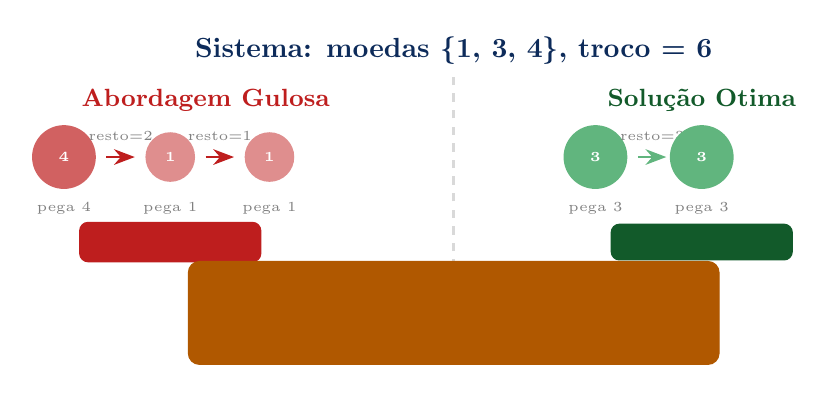
\begin{tikzpicture}[scale=0.90]

    \node[font=\bfseries\normalsize,gemaBlue] at (7.0,5.5)
      {Sistema: moedas \{1, 3, 4\}, troco = 6};

    % ── GULOSO ────────────────────────────────────────────
    \node[font=\bfseries\small,gemaRed] at (3.5,4.8){Abordagem Gulosa};
    % Passo 1: escolhe 4
    \fill[gemaRed!70] (1.5,4.0) circle (0.45);
    \node[font=\bfseries\tiny,white] at (1.5,4.0){4};
    \node[font=\tiny,gray,below] at (1.5,3.5){pega 4};
    \draw[-{Stealth},gemaRed,line width=1pt](2.1,4.0)--(2.5,4.0);
    \node[font=\tiny,gray] at (2.3,4.3){resto=2};
    % Passo 2: escolhe 1
    \fill[gemaRed!50] (3.0,4.0) circle (0.35);
    \node[font=\bfseries\tiny,white] at (3.0,4.0){1};
    \node[font=\tiny,gray,below] at (3.0,3.5){pega 1};
    \draw[-{Stealth},gemaRed,line width=1pt](3.5,4.0)--(3.9,4.0);
    \node[font=\tiny,gray] at (3.7,4.3){resto=1};
    % Passo 3: escolhe 1
    \fill[gemaRed!50] (4.4,4.0) circle (0.35);
    \node[font=\bfseries\tiny,white] at (4.4,4.0){1};
    \node[font=\tiny,gray,below] at (4.4,3.5){pega 1};
    % Resultado ruim
    \node[draw=gemaRed,fill=gemaRed!15,rounded corners=3pt,
          font=\bfseries\small,gemaRed,minimum width=2.3cm] at (3.0,2.8)
      {3 moedas \texttimes};

    % separador
    \draw[gray!30,dashed,line width=1pt](7.0,1.5)--(7.0,5.2);

    % ── ótimo ─────────────────────────────────────────────
    \node[font=\bfseries\small,gemaGreen!60!black] at (10.5,4.8){Solução Otima};
    % Passo 1: escolhe 3
    \fill[gemaGreen!70] (9.0,4.0) circle (0.45);
    \node[font=\bfseries\tiny,white] at (9.0,4.0){3};
    \node[font=\tiny,gray,below] at (9.0,3.5){pega 3};
    \draw[-{Stealth},gemaGreen!70,line width=1pt](9.6,4.0)--(10.0,4.0);
    \node[font=\tiny,gray] at (9.8,4.3){resto=3};
    % Passo 2: escolhe 3
    \fill[gemaGreen!70] (10.5,4.0) circle (0.45);
    \node[font=\bfseries\tiny,white] at (10.5,4.0){3};
    \node[font=\tiny,gray,below] at (10.5,3.5){pega 3};
    % Resultado bom
    \node[draw=gemaGreen,fill=gemaGreen!15,rounded corners=3pt,
          font=\bfseries\small,gemaGreen!60!black,minimum width=2.3cm]
          at (10.5,2.8){2 moedas \checkmark};

    % Mensagem central
    \node[draw=gemaOrange,fill=gemaOrange!10,rounded corners=4pt,
          font=\small,gemaOrange!80!black,
          minimum width=6cm,align=center] at (7.0,1.8)
      {Guloso pegou 4 (localmente ótimo)\\
       mas bloqueou o caminho para o ótimo global!\\
       \textbf{Neste caso: use Programação dinâmica.}};

  \end{tikzpicture}
  \end{adjustbox}
\end{frame}

% ── EXEMPLO 2: INTERVAL SCHEDULING ──────────────────────────
\begin{frame}{Exemplo 2 --- Interval Scheduling (Seleção de Atividades)}
  \begin{columns}[c]
    \column{0.48\textwidth}
      \begin{tcolorbox}[caixaAzul,title={Problema}]
        \small
        Dado um conjunto de atividades com inicio
        e fim, selecione o \textbf{maior numero}
        de atividades \textbf{sem sobreposição}.
      \end{tcolorbox}
      \vspace{0.1cm}
      \begin{tcolorbox}[caixaDourada,title={Estrategia Gulosa}]
        \footnotesize
        \textbf{Sempre escolha a atividade que
        termina mais cedo} e nao conflita com
        a ultima selecionada.\\[4pt]
        Intuição: deixar mais \textbf{espaco livre}
        para atividades futuras.
      \end{tcolorbox}
      \vspace{0.1cm}
      \begin{tcolorbox}[caixaVerde,title={Exchange Argument}]
        \footnotesize
        Se existe outra solução que nao escolhe
        a que termina mais cedo, podemos \textbf{trocar}
        a primeira atividade escolhida por ela
        sem reduzir o total. $\Rightarrow$ Guloso e ótimo!
      \end{tcolorbox}
    \column{0.50\textwidth}
      \centering
      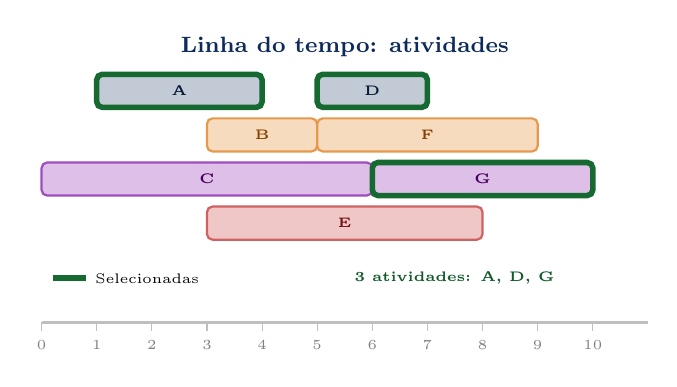
\begin{tikzpicture}[scale=0.70]
        \node[font=\bfseries\footnotesize,gemaBlue] at (5.5,5.0)
          {Linha do tempo: atividades};
        % Eixo do tempo
        \draw[gray!50,line width=1pt](0,0)--(11,0);
        \foreach \x in {0,1,...,10}{
          \draw[gray!50,thin](\x,0)--(\x,-0.15);
          \node[font=\tiny,gray,below] at (\x,-0.15){\x};
        }

        % Atividades (inicio, fim, label, cor, y)
        % A:[1,4], B:[3,5], C:[0,6], D:[5,7], E:[3,8], F:[5,9], G:[6,10]
        \foreach \ini/\fim/\lab/\col/\y in {
          1/4/A/gemaBlue/4.2,
          3/5/B/gemaOrange/3.4,
          0/6/C/gemaPurple/2.6,
          5/7/D/gemaBlue/4.2,
          3/8/E/gemaRed/1.8,
          5/9/F/gemaOrange/3.4,
          6/10/G/gemaPurple/2.6}{
          \draw[fill=\col!25,draw=\col!70,rounded corners=2pt,line width=0.8pt]
            (\ini,\y-0.3) rectangle (\fim,\y+0.3)
            node[midway,font=\bfseries\tiny,\col!60!black]{\lab};
        }
        % Atividades selecionadas (destacadas)
        % A termina em 4, D termina em 7, G termina em 10
        \draw[gemaGreen!70!black,line width=2pt,rounded corners=2pt]
          (1,3.9) rectangle (4,4.5);
        \draw[gemaGreen!70!black,line width=2pt,rounded corners=2pt]
          (5,3.9) rectangle (7,4.5);
        \draw[gemaGreen!70!black,line width=2pt,rounded corners=2pt]
          (6,2.3) rectangle (10,2.9);
        % Legenda
        \draw[gemaGreen!70!black,line width=2pt](0.2,0.8)--(0.8,0.8);
        \node[font=\tiny,right] at (0.8,0.8){Selecionadas};
        \node[font=\tiny,gemaGreen!60!black,right] at (5.5,0.8)
          {\textbf{3 atividades: A, D, G}};
      \end{tikzpicture}
  \end{columns}
\end{frame}

% ── EXEMPLO 2: CÓDIGO ───────────────────────────────────────
\begin{frame}[fragile,shrink=3]{Exemplo 2 --- Codigo C++: Interval Scheduling}
  \begin{columns}[t]
    \column{0.60\textwidth}
      \begin{tcolorbox}[caixaCodigo]
        \begin{lstlisting}[style=cppstyle]
#include <bits/stdc++.h>
using namespace std;

int main(){
    int n;
    cin >> n;
    // Armazena (fim, inicio) para ordenar por fim
    vector<pair<int,int>> atv(n);
    for(auto& [fim, ini] : atv)
        cin >> ini >> fim;

    // CHAVE: ordenar pelo tempo de FIM
    sort(atv.begin(), atv.end());

    int cont = 0;
    int ultimo_fim = -1; // fim da ultima escolhida

    for(auto [fim, ini] : atv){
        // Nao conflita com a ultima selecionada?
        if(ini >= ultimo_fim){
            cont++;
            ultimo_fim = fim;
            // (aqui podemos guardar quais foram)
        }
    }

    cout << "Max atividades: " << cont << "\n";
    return 0;
}
        \end{lstlisting}
      \end{tcolorbox}
    \column{0.38\textwidth}
      \begin{tcolorbox}[caixaDourada,title={Passos do algoritmo}]
        \begin{enumerate}\footnotesize
          \item Leia os intervalos
          \item \textbf{Ordene pelo tempo de fim}
          \item Percorra: se inicio $\geq$ ultimo fim, seleciona
          \item Atualize ultimo fim
        \end{enumerate}
      \end{tcolorbox}
      \vspace{0.1cm}
      \begin{tcolorbox}[caixaAzul,title={Complexidade}]
        \footnotesize
        \textbf{Ordenação:} O(n log n)\\
        \textbf{Seleção:} O(n)\\
        \textbf{Total:} \textbf{O(n log n)}
      \end{tcolorbox}
      \vspace{0.1cm}
      \begin{tcolorbox}[caixaVermelho,title={Erro comum}]
        \footnotesize
        Ordenar pelo \textbf{inicio} ou pela
        \textbf{duração} nao garante otimalidade!\\[3pt]
        Sempre ordene pelo \textbf{fim}.
      \end{tcolorbox}
  \end{columns}
\end{frame}

% ── EXEMPLO 3: PLATAFORMAS / SALAS ──────────────────────────
\begin{frame}{Exemplo 3 --- Minimo de Plataformas / Salas}
  \begin{columns}[c]
    \column{0.48\textwidth}
      \begin{tcolorbox}[caixaAzul,title={Problema}]
        \small
        Dado $n$ trens com horario de chegada e partida,
        qual o \textbf{minimo de plataformas} para
        que nenhum trem fique sem lugar?\\[4pt]
        Equivalente: minimo de salas de reuniao.
      \end{tcolorbox}
      \vspace{0.1cm}
      \begin{tcolorbox}[caixaDourada,title={Estrategia Gulosa}]
        \footnotesize
        \begin{enumerate}\footnotesize
          \item Separe os eventos de \textbf{chegada} e \textbf{partida}
          \item Ordene cada lista separadamente
          \item Use dois ponteiros: ao chegar abre uma sala,
                ao partir fecha; rastreie o maximo simultaneo
        \end{enumerate}
      \end{tcolorbox}
      \vspace{0.1cm}
      \begin{tcolorbox}[caixaVerde,title={Intuição}]
        \footnotesize
        O pico de \textbf{ocupação simultanea}
        determina o minimo de plataformas.\\
        Guloso: processe chegadas e partidas
        em ordem cronologica.
      \end{tcolorbox}
    \column{0.50\textwidth}
      \centering
      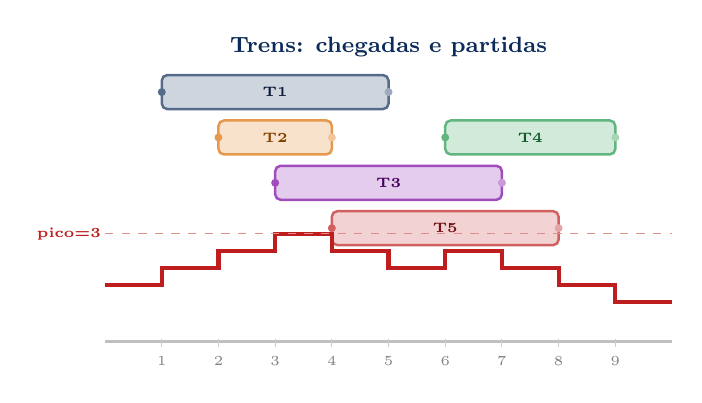
\begin{tikzpicture}[scale=0.72]
        \node[font=\bfseries\footnotesize,gemaBlue] at (5,5.2)
          {Trens: chegadas e partidas};
        % Eixo
        \draw[gray!50,line width=1pt](0,0)--(10,0);
        \foreach \x in {1,2,...,9}{
          \draw[gray!40,thin](\x,0.05)--(\x,-0.1);
          \node[font=\tiny,gray,below] at (\x,-0.1){\x};
        }
        % Trens
        \foreach \ini/\fim/\col/\y/\lab in {
          1/5/gemaBlue/4.4/T1,
          2/4/gemaOrange/3.6/T2,
          3/7/gemaPurple/2.8/T3,
          6/9/gemaGreen/3.6/T4,
          4/8/gemaRed/2.0/T5}{
          \draw[fill=\col!20,draw=\col!70,rounded corners=2pt,line width=0.9pt]
            (\ini,\y-0.3) rectangle (\fim,\y+0.3)
            node[midway,font=\bfseries\tiny,\col!60!black]{\lab};
          \fill[\col!70] (\ini,\y) circle (2pt);
          \fill[\col!40] (\fim,\y) circle (2pt);
        }
        % Grafico de ocupação
        \draw[gemaRed,line width=1.5pt]
          (0,1.0)--(1,1.0)--(1,1.3)--(2,1.3)--(2,1.6)
          --(3,1.6)--(3,1.9)--(4,1.9)--(4,1.6)
          --(5,1.6)--(5,1.3)--(6,1.3)--(6,1.6)
          --(7,1.6)--(7,1.3)--(8,1.3)--(8,1.0)
          --(9,1.0)--(9,0.7)--(10,0.7);
        \node[font=\tiny,gemaRed,left] at (0.1,1.9)
          {\textbf{pico=3}};
        \draw[gemaRed!50,dashed,thin](0,1.9)--(10,1.9);
      \end{tikzpicture}
      \begin{tcolorbox}[caixaAmarelo,title={Resposta}]
        \footnotesize
        Pico = 3 trens simultaneos $\Rightarrow$
        precisamos de \textbf{3 plataformas}.
      \end{tcolorbox}
  \end{columns}
\end{frame}

% ── EXEMPLO 3: CÓDIGO ───────────────────────────────────────
\begin{frame}[fragile,shrink=3]{Exemplo 3 --- Codigo C++: Minimo de Plataformas}
  \begin{columns}[t]
    \column{0.60\textwidth}
      \begin{tcolorbox}[caixaCodigo]
        \begin{lstlisting}[style=cppstyle]
#include <bits/stdc++.h>
using namespace std;

int main(){
    int n; cin >> n;
    vector<int> cheg(n), part(n);
    for(int i = 0; i < n; i++)
        cin >> cheg[i] >> part[i];

    // Ordena chegadas e partidas separadamente
    sort(cheg.begin(), cheg.end());
    sort(part.begin(), part.end());

    int plat = 0, maximo = 0;
    int i = 0, j = 0;

    // Dois ponteiros: percorre eventos em ordem
    while(i < n && j < n){
        if(cheg[i] < part[j]){
            plat++;          // chegou novo trem
            maximo = max(maximo, plat);
            i++;
        } else {
            plat--;          // trem partiu
            j++;
        }
    }

    cout << "Plataformas necessarias: " << maximo << "\n";
    return 0;
}
        \end{lstlisting}
      \end{tcolorbox}
    \column{0.38\textwidth}
      \begin{tcolorbox}[caixaDourada,title={Dois Ponteiros}]
        \footnotesize
        \texttt{i} percorre chegadas\\
        \texttt{j} percorre partidas\\[4pt]
        Quem vem primeiro (cronolog.):
        \begin{itemize}\footnotesize
          \item chegada $\to$ \texttt{plat++}
          \item partida  $\to$ \texttt{plat--}
        \end{itemize}
      \end{tcolorbox}
      \vspace{0.1cm}
      \begin{tcolorbox}[caixaAzul,title={Complexidade}]
        \footnotesize
        \textbf{Ordenação:} O(n log n)\\
        \textbf{Varredura:} O(n)\\
        \textbf{Total:} \textbf{O(n log n)}
      \end{tcolorbox}
      \vspace{0.1cm}
      \begin{tcolorbox}[caixaVerde,title={Aplicacoes}]
        \footnotesize
        Salas de reuniao\\
        Alocação de recursos\\
        Conflito de jobs\\
        Servidores simultaneos
      \end{tcolorbox}
  \end{columns}
\end{frame}

% ── EXEMPLO 4: FRACTIONAL KNAPSACK ──────────────────────────
\begin{frame}{Exemplo 4 --- Mochila Fracionaria (Fractional Knapsack)}
  \begin{columns}[c]
    \column{0.48\textwidth}
      \begin{tcolorbox}[caixaAzul,title={Problema}]
        \small
        Mochila com capacidade $W$.\\
        Itens com \textbf{peso} $w_i$ e \textbf{valor} $v_i$.\\
        \textbf{Pode-se fracionr} os itens.\\
        Maximizar o valor total carregado.
      \end{tcolorbox}
      \vspace{0.1cm}
      \begin{tcolorbox}[caixaDourada,title={Estrategia Gulosa}]
        \footnotesize
        Ordene os itens por
        \textbf{valor por unidade de peso}
        ($v_i / w_i$) em ordem \textbf{decrescente}.\\[3pt]
        Pegue o maximo possivel de cada item,
        comecando pelo de maior ``densidade''.
      \end{tcolorbox}
      \vspace{0.1cm}
      \begin{tcolorbox}[caixaVermelho,title={Diferenca para 0/1 Knapsack}]
        \footnotesize
        \textbf{Fracionario:} guloso e \textbf{ótimo}\\
        (pode pegar fatias)\\[3pt]
        \textbf{0/1 Knapsack:} guloso \textbf{nao} e ótimo\\
        (item inteiro ou nenhum) $\to$ use DP!
      \end{tcolorbox}
    \column{0.50\textwidth}
      \centering
      % Tabela de itens e visualização
      \begin{tikzpicture}[scale=0.75]
        \node[font=\bfseries\footnotesize,gemaBlue] at (3.5,5.0)
          {Capacidade W = 50};

        % Tabela
        \node[font=\tiny\bfseries,gemaBlue] at (0.5,4.4){Item};
        \node[font=\tiny\bfseries,gemaBlue] at (1.6,4.4){Peso};
        \node[font=\tiny\bfseries,gemaBlue] at (2.7,4.4){Valor};
        \node[font=\tiny\bfseries,gemaBlue] at (3.9,4.4){v/w};
        \node[font=\tiny\bfseries,gemaGold] at (5.1,4.4){Ordem};
        \draw[gemaBlue!40,thin](0,4.15)--(5.5,4.15);

        \foreach \it/\pe/\va/\ratio/\ord/\y/\col in {
          A/10/60/6.0/1/3.6/gemaGreen,
          B/20/100/5.0/2/2.8/gemaBlue,
          C/30/120/4.0/3/2.0/gemaOrange,
          D/10/30/3.0/4/1.2/gemaRed}{
          \node[font=\tiny] at (0.5,\y){\it};
          \node[font=\tiny] at (1.6,\y){\pe};
          \node[font=\tiny] at (2.7,\y){\va};
          \node[font=\tiny,\col!70!black,bfseries] at (3.9,\y){\ratio};
          \node[font=\bfseries\tiny,gemaGold!70!black] at (5.1,\y){\ord};
        }

        % Mochila visual
        \node[font=\tiny\bfseries,gemaBlue] at (3.5,0.8){Preenchimento da mochila};
        \draw[gemaBlue!40,rounded corners=2pt,line width=1pt](0.5,-0.1) rectangle (6.5,0.5);

        % Item A: 10/50 = 20% da barra, valor 60
        \draw[fill=gemaGreen!50,draw=gemaGreen!70,rounded corners=1pt]
          (0.5,-0.1) rectangle (1.7,0.5);
        \node[font=\tiny,white] at (1.1,0.2){A(10)};

        % Item B: 20/50 = 40%, valor 100
        \draw[fill=gemaBlue!50,draw=gemaBlue!70,rounded corners=1pt]
          (1.7,-0.1) rectangle (4.1,0.5);
        \node[font=\tiny,white] at (2.9,0.2){B(20)};

        % Item C: 20/50 fracionado, valor 80
        \draw[fill=gemaOrange!50,draw=gemaOrange!70,rounded corners=1pt]
          (4.1,-0.1) rectangle (6.5,0.5);
        \node[font=\tiny,white] at (5.3,0.2){C(20)};

        % Total
        \node[font=\bfseries\tiny,gemaGold!70!black] at (3.5,-0.5)
          {Total: 60+100+80=\textbf{240} (C fracionado em 20/30)};
      \end{tikzpicture}
  \end{columns}
\end{frame}

% ── EXEMPLO 4: CÓDIGO ───────────────────────────────────────
\begin{frame}[fragile,shrink=3]{Exemplo 4 --- Codigo C++: Mochila Fracionaria}
  \begin{columns}[t]
    \column{0.60\textwidth}
      \begin{tcolorbox}[caixaCodigo]
        \begin{lstlisting}[style=cppstyle]
#include <bits/stdc++.h>
using namespace std;

struct Item {
    double peso, valor;
    double ratio() const { return valor / peso; }
};

int main(){
    int n; double W;
    cin >> n >> W;

    vector<Item> itens(n);
    for(auto& it : itens)
        cin >> it.peso >> it.valor;

    // CHAVE: ordenar por valor/peso (decrescente)
    sort(itens.begin(), itens.end(),
         [](const Item& a, const Item& b){
             return a.ratio() > b.ratio();
         });

    double totalValor = 0.0;

    for(auto& it : itens){
        if(W <= 0) break;
        double pegar = min(it.peso, W);
        totalValor += pegar * it.ratio();
        W -= pegar;
    }

    cout << fixed << setprecision(2)
         << "Valor maximo: " << totalValor << "\n";
    return 0;
}
        \end{lstlisting}
      \end{tcolorbox}
    \column{0.38\textwidth}
      \begin{tcolorbox}[caixaDourada,title={Por que funciona?}]
        \footnotesize
        Pegando sempre a maior
        ``densidade'' ($v/w$), maximizamos
        valor por unidade de espaco.\\[4pt]
        Como \textbf{podemos fracionr},
        nao há perda ao dividir o ultimo item.
      \end{tcolorbox}
      \vspace{0.1cm}
      \begin{tcolorbox}[caixaAzul,title={Complexidade}]
        \footnotesize
        \textbf{Ordenação:} O(n log n)\\
        \textbf{Preenchimento:} O(n)\\
        \textbf{Total:} \textbf{O(n log n)}
      \end{tcolorbox}
      \vspace{0.1cm}
      \begin{tcolorbox}[caixaVermelho,title={0/1 Knapsack}]
        \footnotesize
        Se os itens sao \textbf{inteiros}
        (nao pode fracionr), o guloso
        \textbf{nao e ótimo}.\\[2pt]
        Use DP com tabela $n \times W$.
      \end{tcolorbox}
  \end{columns}
\end{frame}

% ============================================================
%  PARTE 3 — ESTRATEGIAS E PRATICA
% ============================================================
{
\setbeamertemplate{footline}{}
\begin{frame}[noframenumbering]
  \centering\vspace{1.0cm}
  {\fontsize{36}{44}\selectfont\bfseries\color{gemaBlue} 3}\par
  \vspace{0.25cm}
  {\Large\color{greedyGold}\bfseries Estrategias e Pratica}\par
  \vspace{0.15cm}
  {\color{gray}\small Tecnicas $\cdot$ Como identificar $\cdot$ Armadilhas $\cdot$ Exercicios}
\end{frame}
}

% ── ESTRATEGIAS COMUNS ──────────────────────────────────────
\begin{frame}[shrink=2]{Estrategias Comuns em Algoritmos Gulosos}
  \begin{columns}[t]
    \column{0.48\textwidth}
      \begin{tcolorbox}[caixaDourada,title={1. Ordenar e Varrer}]
        \footnotesize
        A mais comum! Ordene por algum criterio
        que reflita a ``qualidade'' de cada escolha.\\[3pt]
        \textbf{Exemplos:}
        \begin{itemize}\footnotesize
          \item Interval Scheduling: ordenar por fim
          \item Mochila Fracionaria: ordenar por v/w
          \item Troco: ordenar por valor (desc.)
        \end{itemize}
      \end{tcolorbox}
      \vspace{0.1cm}
      \begin{tcolorbox}[caixaRoxa,title={2. Priority Queue (Heap)}]
        \footnotesize
        Quando a ``melhor escolha'' muda dinâmicamente
        conforme processamos os elementos.\\[3pt]
        \textbf{Exemplos:}
        \begin{itemize}\footnotesize
          \item Huffman Coding: sempre junta os 2 menores
          \item Job Scheduling: menor deadline primeiro
          \item Prim's MST: menor aresta disponivel
        \end{itemize}
      \end{tcolorbox}
    \column{0.48\textwidth}
      \begin{tcolorbox}[caixaVerde,title={3. Dois Ponteiros}]
        \footnotesize
        Dois indices percorrendo arrays ordenados
        em direcoes ou velocidades distintas.\\[3pt]
        \textbf{Exemplos:}
        \begin{itemize}\footnotesize
          \item Minimo de Plataformas: chegadas vs partidas
          \item Matching de pares
          \item Two Sum em array ordenado
        \end{itemize}
      \end{tcolorbox}
      \vspace{0.1cm}
      \begin{tcolorbox}[caixaLaranja,title={4. Intercambio (Exchange)}]
        \footnotesize
        Tecnica de prova: mostrar que qualquer
        desvio da escolha gulosa pode ser
        ``trocado'' sem piorar.\\[3pt]
        \textbf{Padrao da prova:}\\
        Tome sol. otima $\neq$ gulosa $\Rightarrow$ troque
        o primeiro ponto de diferenca $\Rightarrow$
        nao piora $\Rightarrow$ guloso e ótimo.
      \end{tcolorbox}
  \end{columns}
\end{frame}

% ── COMO IDENTIFICAR ────────────────────────────────────────
\begin{frame}{Como Identificar Problemas Gulosos na OBI?}
  \begin{columns}[t]
    \column{0.47\textwidth}
      \begin{block}{Sinais de alerta para Guloso}
        \begin{itemize}\footnotesize
          \item ``\textbf{Maximo} de atividades / eventos''
          \item ``\textbf{Minimo} de recursos / salas''
          \item ``\textbf{Ordenar} algo para otimizar''
          \item ``Cada decisao e \textbf{independente}''
          \item ``\textbf{Sem possibilidade} de revisitar''
          \item Constraints $n \leq 10^6$: O(n log n) necessario
        \end{itemize}
      \end{block}
      \vspace{0.1cm}
      \begin{tcolorbox}[caixaLaranja,title={Palavras-chave tipicas}]
        \footnotesize
        ``maximize'', ``minimize'', ``selecione o maior numero'',
        ``menor numero de'', ``intervalo'', ``atividade'',
        ``plataforma'', ``sala'', ``fracionario'', ``troco''
      \end{tcolorbox}
    \column{0.50\textwidth}
      \begin{tcolorbox}[caixaVermelho,title={Quando NAO usar Guloso}]
        \begin{itemize}\footnotesize
          \item Decisao atual depende de \textbf{escolhas futuras}
          \item Contraexemplo simples existe (teste!)
          \item Problema pede \textbf{0/1} (inteiro, nao fracionario)
          \item Contagem de caminhos / solucoes
          \item Jogos com adversario
        \end{itemize}
      \end{tcolorbox}
      \vspace{0.1cm}
      \begin{tcolorbox}[caixaDourada,title={Receita para a prova}]
        \footnotesize
        \begin{enumerate}\footnotesize
          \item Pense na escolha gulosa
          \item Teste com 2-3 exemplos pequenos
          \item Tente construir um \textbf{contraexemplo}
          \item Se nao encontrar: implemente e submeta
          \item WA? Busque o contraexemplo ou mude para DP
        \end{enumerate}
      \end{tcolorbox}
  \end{columns}
\end{frame}

% ── ARMADILHAS ──────────────────────────────────────────────
\begin{frame}{Armadilhas Comuns em Competicoes}
  \centering
  \begin{adjustbox}{max totalsize={0.96\textwidth}{0.78\textheight},center}
  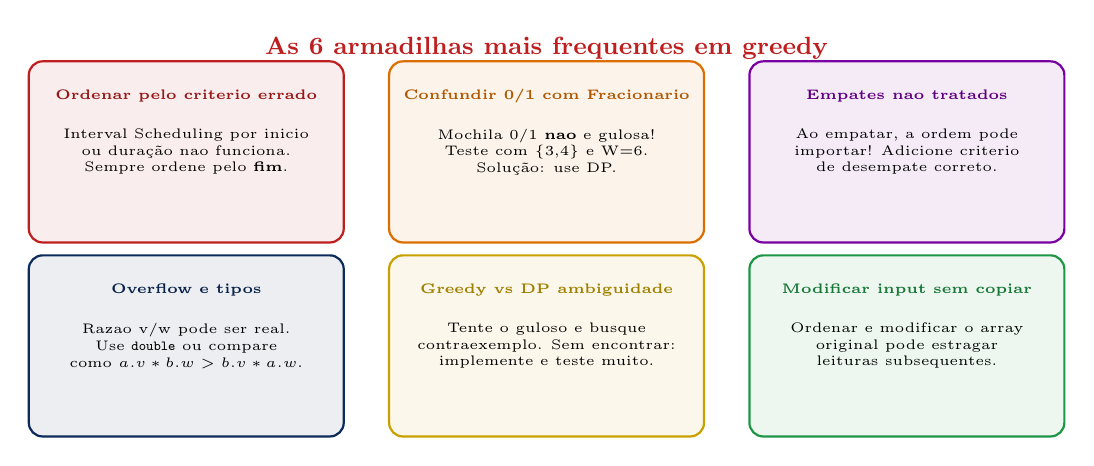
\begin{tikzpicture}[scale=0.88]

    % Caixas de armadilhas
    \foreach \x/\y/\title/\desc/\cor in {
      1.8/3.8/{Ordenar pelo criterio errado}/{Interval Scheduling por inicio\\ou duração nao funciona.\\Sempre ordene pelo \textbf{fim}.}/gemaRed,
      7.0/3.8/{Confundir 0/1 com Fracionario}/{Mochila 0/1 \textbf{nao} e gulosa!\\Teste com \{3,4\} e W=6.\\Solução: use DP.}/gemaOrange,
      12.2/3.8/{Empates nao tratados}/{Ao empatar, a ordem pode\\importar! Adicione criterio\\de desempate correto.}/gemaPurple,
      1.8/1.0/{Overflow e tipos}/{Razao v/w pode ser real.\\Use \texttt{double} ou compare\\como $a.v*b.w > b.v*a.w$.}/gemaBlue,
      7.0/1.0/{Greedy vs DP ambiguidade}/{Tente o guloso e busque\\contraexemplo. Sem encontrar:\\implemente e teste muito.}/gemaGold,
      12.2/1.0/{Modificar input sem copiar}/{Ordenar e modificar o array\\original pode estragar\\leituras subsequentes.}/gemaGreen}{
      \node[draw=\cor,fill=\cor!8,rounded corners=5pt,
            minimum width=4.0cm,minimum height=2.3cm,
            text width=3.6cm,align=center,
            font=\tiny,line width=0.8pt] at (\x,\y){};
      \node[font=\bfseries\tiny,\cor!80!black,align=center] at (\x,\y+0.8){\title};
      \node[font=\tiny,align=center] at (\x,\y){\desc};
    }

    % Titulo
    \node[font=\bfseries\small,gemaRed] at (7.0,5.3)
      {As 6 armadilhas mais frequentes em greedy};

  \end{tikzpicture}
  \end{adjustbox}
\end{frame}

% ── COMPARAção BFS VS GULOSO ────────────────────────────────
\begin{frame}{Comparação: Paradigmas de Solução}
  \begin{tcolorbox}[caixaAzul,title={Quando usar cada paradigma?}]
    \centering\footnotesize
    \begin{tabular}{lcccc}
      \toprule
      \textbf{Criterio} & \textbf{Forca Bruta} & \textbf{Rec./Backtrack} & \textbf{Prog. dinâmica} & \textbf{Guloso}\\
      \midrule
      Corretude    & Sempre & Sempre & Sempre* & Se provar\\
      Complexidade & $2^n$/$n!$ & exp & poli. & O(n log n)\\
      Implementação& Simples & Media & Media & Simples\\
      n maximo     & $\leq$20 & $\leq$30 & $\leq$10$^4$ & $\leq$10$^6$\\
      Revisita?    & Sim & Sim & Sim & Nao\\
      \bottomrule
    \end{tabular}
  \end{tcolorbox}
  \vspace{0.12cm}
  \begin{columns}[t]
    \column{0.32\textwidth}
      \begin{tcolorbox}[caixaVermelho,title={Forca Bruta}]
        \footnotesize
        Use quando $n \leq 20$ e\\
        nao há outra saida.\\
        Util para \textbf{testar} solucoes.
      \end{tcolorbox}
    \column{0.32\textwidth}
      \begin{tcolorbox}[caixaAzul,title={Programação dinâmica}]
        \footnotesize
        Quando há \textbf{sobreposição}\\
        de subproblemas e nao\\
        há escolha gulosa clara.
      \end{tcolorbox}
    \column{0.32\textwidth}
      \begin{tcolorbox}[caixaDourada,title={Guloso}]
        \footnotesize
        Quando decisao local\\
        nao compromete o futuro\\
        e pode ser \textbf{provado}.
      \end{tcolorbox}
  \end{columns}
\end{frame}

% ── PROBLEMAS CLASSICOS ─────────────────────────────────────
\begin{frame}{Problemas Classicos para Praticar}
  \begin{columns}[t]
    \column{0.48\textwidth}
      \begin{tcolorbox}[caixaVerde,title={Iniciante}]
        \begin{itemize}\footnotesize
          \item \textbf{SPOJ COINS} --- Troco de moedas canonico
          \item \textbf{CF 670C} --- Cinema (ordenar por tipo)
          \item \textbf{CF 1130A} --- Be Positive (guloso simples)
          \item \textbf{OBI 2018} --- Alocação de salas
          \item \textbf{NEPS} --- Agenda de atividades
        \end{itemize}
      \end{tcolorbox}
      \vspace{0.1cm}
      \begin{tcolorbox}[caixaAzul,title={Intermediario}]
        \begin{itemize}\footnotesize
          \item \textbf{CF 1481C} --- Skyscrapers (escolha de pico)
          \item \textbf{CF 1353D} --- Intervals (guloso com PQ)
          \item \textbf{LC 435} --- Non-overlapping Intervals
          \item \textbf{CF 455A} --- Boredom (ordenar e somar)
        \end{itemize}
      \end{tcolorbox}
    \column{0.48\textwidth}
      \begin{tcolorbox}[caixaRoxa,title={Avancado}]
        \begin{itemize}\footnotesize
          \item \textbf{CF 1244C} --- Combining Olympiads
          \item \textbf{CF 1369C} --- RLE String (guloso + analise)
          \item \textbf{CF 1537C} --- Challenging Cliffs (guloso criativo)
          \item \textbf{LC 406} --- Queue Reconstruction by Height
        \end{itemize}
      \end{tcolorbox}
      \vspace{0.1cm}
      \begin{tcolorbox}[caixaAmarelo,title={Dica de estudo}]
        \footnotesize
        Para cada problema:\\
        \begin{enumerate}\footnotesize
          \item Pense no criterio de ordenação
          \item Prove por exchange argument
          \item Implemente e submeta
          \item Analise os casos de erro
        \end{enumerate}
      \end{tcolorbox}
  \end{columns}
\end{frame}

% ── RESUMO VISUAL ───────────────────────────────────────────
\begin{frame}[shrink=2]{Resumo Geral --- Algoritmos Gulosos}
  \begin{columns}[t]
    \column{0.31\textwidth}
      \begin{block}{O que e?}
        \begin{itemize}\footnotesize
          \item Escolha localmente otima
          \item Sem revisitar decisoes
          \item Nao e sempre correto
          \item Geralmente O(n log n)
        \end{itemize}
      \end{block}
      \vspace{0.1cm}
      \begin{block}{Propriedades}
        \begin{itemize}\footnotesize
          \item Greedy Choice Property
          \item Optimal Substructure
          \item Prova: exchange argument
        \end{itemize}
      \end{block}
    \column{0.31\textwidth}
      \begin{block}{Exemplos vistos}
        \begin{itemize}\footnotesize
          \item Troco (moedas canonicas)
          \item Interval Scheduling
          \item Minimo de Plataformas
          \item Mochila Fracionaria
        \end{itemize}
      \end{block}
      \vspace{0.1cm}
      \begin{block}{Tecnicas}
        \begin{itemize}\footnotesize
          \item Ordenar e varrer
          \item Priority Queue
          \item Dois ponteiros
          \item Exchange argument
        \end{itemize}
      \end{block}
    \column{0.31\textwidth}
      \begin{tcolorbox}[caixaDourada,title={Regra de Ouro}]
        \footnotesize
        \textbf{1.} Identifique a ``melhor escolha local''\\[3pt]
        \textbf{2.} Ordene por esse criterio\\[3pt]
        \textbf{3.} Teste casos pequenos\\[3pt]
        \textbf{4.} Busque contraexemplo\\[3pt]
        \textbf{5.} Se nao achar: implemente!\\[3pt]
        \textbf{6.} WA? Tente DP ou revise a prova
      \end{tcolorbox}
      \vspace{0.1cm}
      \begin{tcolorbox}[caixaVermelho,title={Nunca esqueca}]
        \footnotesize
        Contra-provar e tao\\
        importante quanto provar!\\
        Moedas \{1,3,4\}, troco=6:\\
        Guloso $\to$ ERRADO.
      \end{tcolorbox}
  \end{columns}
\end{frame}

% ── SLIDE FINAL ─────────────────────────────────────────────
{
\setbeamertemplate{footline}{}
\begin{frame}[noframenumbering]
  \centering\vspace{0.1cm}
  \begin{columns}[c]
    \column{0.28\textwidth}
      \centering
\includegraphics[width=0.65\linewidth]{logo.png}
    \column{0.42\textwidth}
      \centering
      {\large\color{gemaBlue}\bfseries Bons estudos\\e boa prova!}\par
      \vspace{0.1cm}
      {\small\color{gemaCyan} GEMA --- Maratonas de Programação}\par
      \vspace{0.1cm}
      {\footnotesize\color{gray} Proxima aula: Programação dinâmica}
    \column{0.28\textwidth}
      \centering
\includegraphics[width=0.65\linewidth]{logo_obi.png}
  \end{columns}
  \vspace{0.18cm}

\end{frame}
}

\end{document}